\RequirePackage{luatex85}
\documentclass[border=1pt]{standalone}

\usepackage{tikz}
\usetikzlibrary{arrows, patterns}

\def\hexagonsize{0.5cm}
\pgfdeclarepatternformonly
	{hexagons}% name
	{\pgfpointorigin}% lower left
	{\pgfpoint{3*\hexagonsize}{0.866025*2*\hexagonsize}}%  upper right
	{\pgfpoint{3*\hexagonsize}{0.866025*2*\hexagonsize}}%  tile size
	{% shape description
	  \pgfsetlinewidth{0.4pt}
	  \pgftransformshift{\pgfpoint{0mm}{0.866025*\hexagonsize}}
	  \pgfpathmoveto{\pgfpoint{0mm}{0mm}}
	  \pgfpathlineto{\pgfpoint{0.5*\hexagonsize}{0mm}}
	  \pgfpathlineto{\pgfpoint{\hexagonsize}{-0.866025*\hexagonsize}}
	  \pgfpathlineto{\pgfpoint{2*\hexagonsize}{-0.866025*\hexagonsize}}
	  \pgfpathlineto{\pgfpoint{2.5*\hexagonsize}{0mm}}
	  \pgfpathlineto{\pgfpoint{3*\hexagonsize+0.2mm}{0mm}}
	  \pgfpathmoveto{\pgfpoint{0.5*\hexagonsize}{0mm}}
	  \pgfpathlineto{\pgfpoint{\hexagonsize}{0.866025*\hexagonsize}}
	  \pgfpathlineto{\pgfpoint{2*\hexagonsize}{0.866025*\hexagonsize}}
	  \pgfpathlineto{\pgfpoint{2.5*\hexagonsize}{0mm}}
	  \pgfusepath{stroke}
	}

\tikzstyle{distArrow} = [<<->>, shorten >=8pt, shorten <=8pt, thick, line width=4pt]
\tikzstyle{dist2Arrow} = [|<->|, thick, line width=4pt]
\tikzstyle{pointer} = [->, shorten >=8pt, shorten <=14pt, thick, line width=2pt]
\tikzstyle{textStyle} = [fill=white!90!black]


\begin{document}
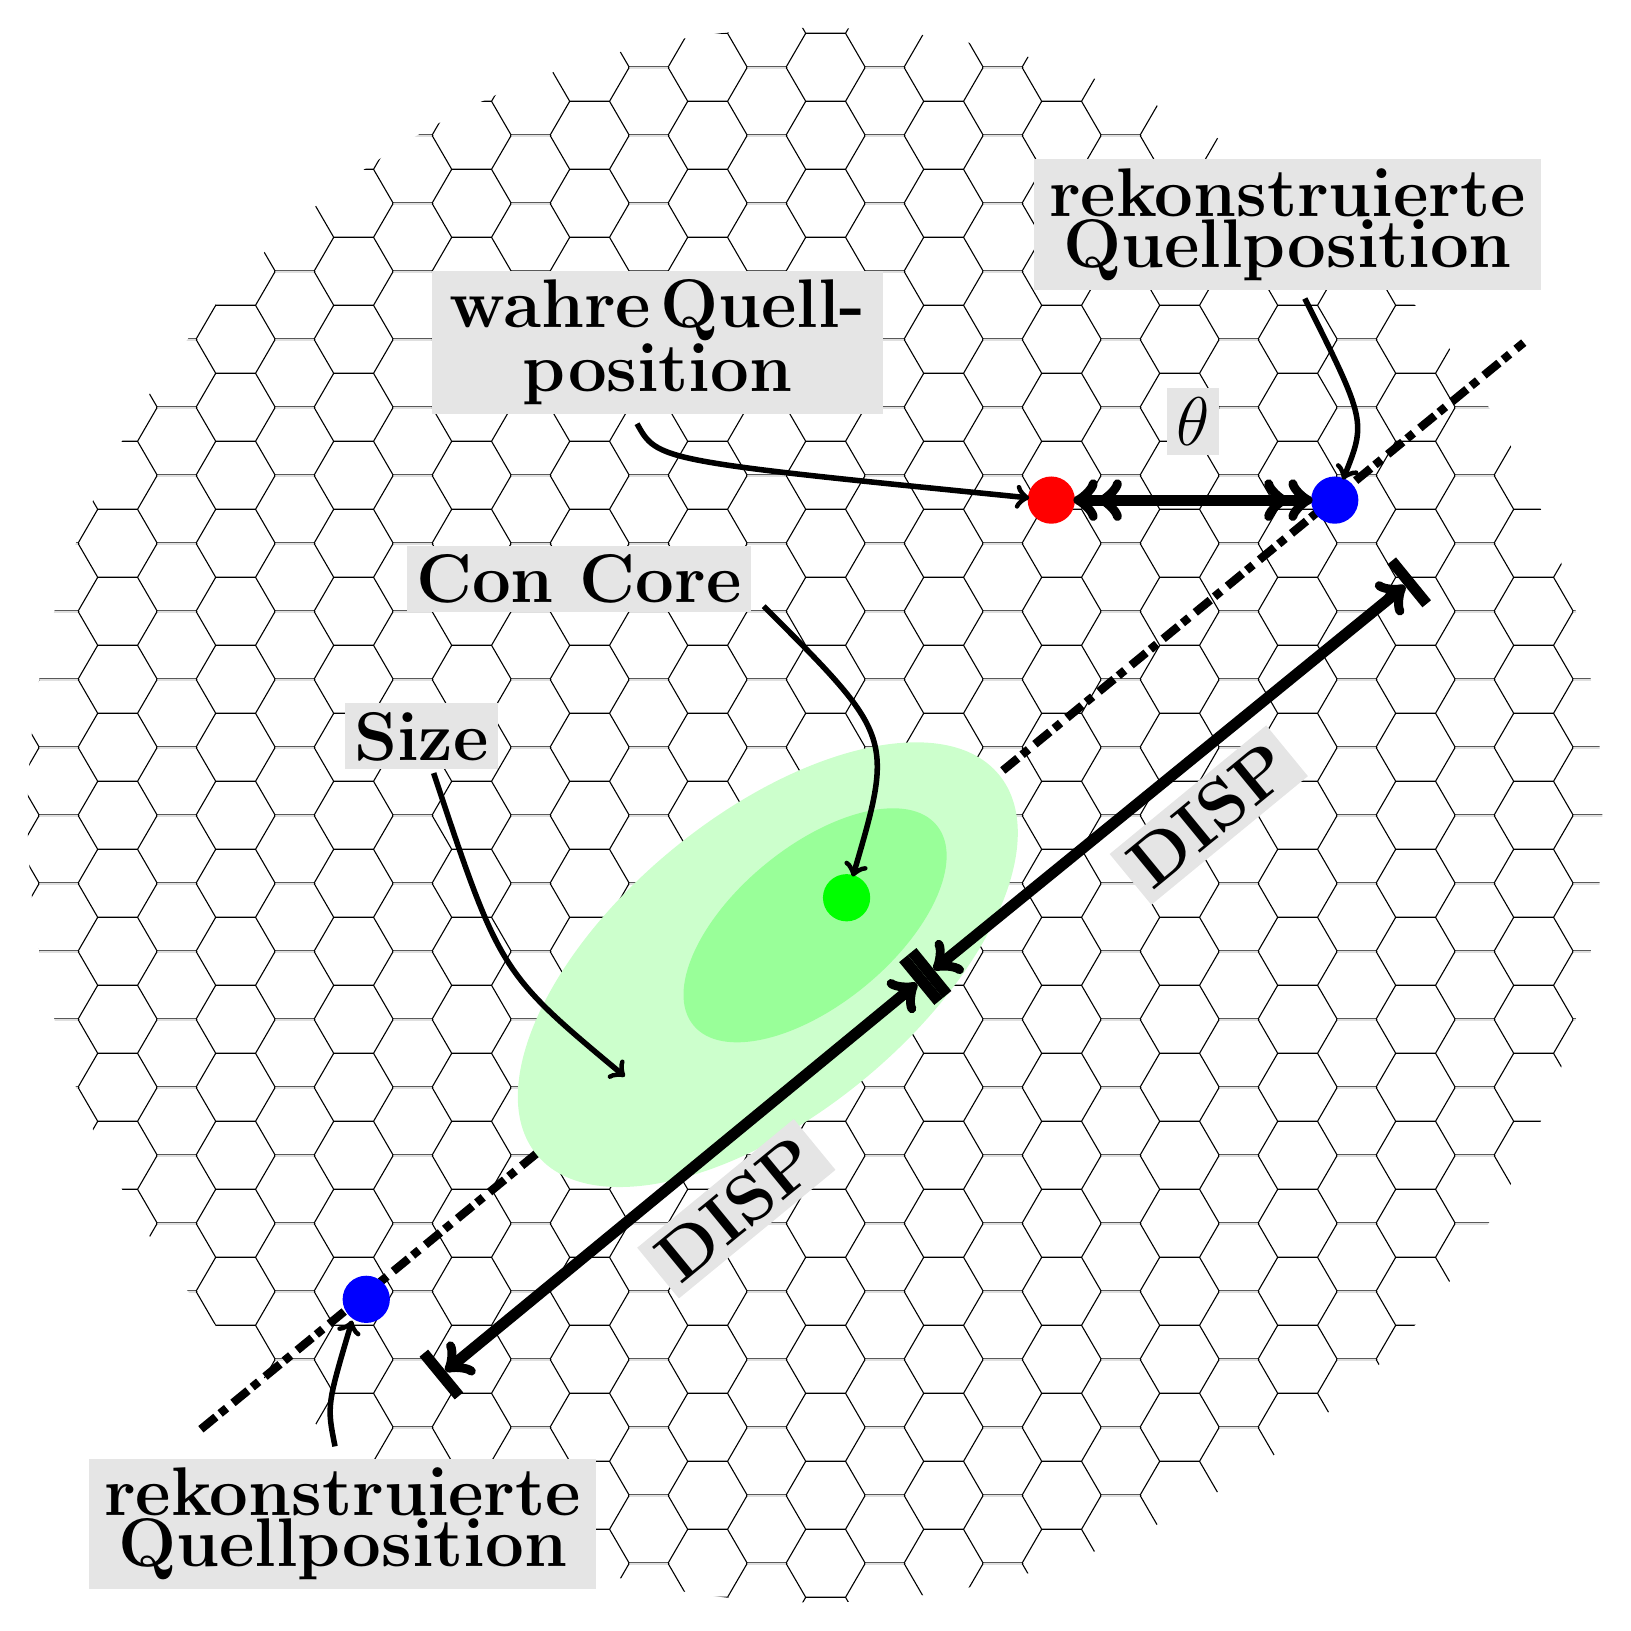
\begin{tikzpicture}
  %camera Achse
  \draw[line width=3pt,,dash pattern={on 7pt off 2pt on 3pt off 3pt}] (-7.8,-7.8) -- (9,6);
  %zeichnet hexagonales Rundes Grid
  \fill[pattern=hexagons] (0,0) circle (10cm);

  %position expected source
  \fill[fill=blue] (6.6, 4) circle [radius=0.3];
  %position measured source 
  \fill[fill=red] (3,4) circle [radius=0.3];
  %theta2
  \draw[distArrow] (3,4) -- (6.6,4);

  % Con core of image 
  \fill[fill=green!20] (-0.6,-1.9) circle [x radius=38mm, y radius=19mm, rotate=39.4];
  \fill[fill=green!40] (0,-1.4) circle [x radius=20mm, y radius=10mm, rotate=39.4];
  \fill[fill=green] (0.4, -1.05) circle [radius=0.3];
  
  %Vorzeichen
  \fill[fill=blue] (-5.7, -6.15) circle [radius=0.3];

  %DISP
  \draw[dist2Arrow] (7.6,3) -- (1.4,-2.05);
  \draw[dist2Arrow] (1.4,-2.05) -- (-4.8,-7.15);

  %Beschriftung der Sachen
  \node[rotate=39.4, textStyle] at (5,-0) {\Huge \textbf{DISP}};
  \node[rotate=39.4, textStyle] at (-1,-5) {\Huge \textbf{DISP}};
  \node[textStyle] at (4.8,5) {\Huge \textbf{$\theta$}};
  \node[textStyle] at (-3,3) {\Huge \textbf{Con Core}};
  \node[textStyle] at (-5,1) {\Huge \textbf{Size}};
  \node[textStyle, align=center, text width=6.2cm] at (-6,-9) {\Huge \textbf{rekonstruierte Quellposition}};
  \node[textStyle, align=center, text width=6.2cm] at (6,7.5) {\Huge \textbf{rekonstruierte Quellposition}};
  \node[textStyle, align=center, text width=5.5cm] at (-2,6) {\Huge \textbf{wahre Quellposition}};

  %Arrows
  \draw[pointer] (-6,-8.5) .. controls (-6.2,-7.5) .. (-5.8,-6.15);
  \draw[pointer] (6,7.0) .. controls (7,5) .. (6.6,4);
  \draw[pointer] (-5,1) .. controls (-4,-2) .. (-2.2,-3.5);
  \draw[pointer] (-1,3) .. controls (1,1) .. (0.4,-1.05);
  \draw[pointer] (-2.5,5.4) .. controls (-2,4.5) .. (3,4);
  %\draw[dist2Arrow] (1.4,-2.05) -- (-4.8,-7.15);


\end{tikzpicture}
\end{document}
